%%%%%%%%%%%%%%%%%%%%%%%%%%
% BITTE IN UTF-8 OEFFNEN %
%%%%%%%%%%%%%%%%%%%%%%%%%%
\documentclass[xcolor={usenames,dvipsnames}, compress, 10pt]{beamer}

\usepackage[ngerman] {babel}
\usepackage[utf8] {inputenc}

\usepackage{tikz}
\usepackage{graphics}
\usepackage{BeamerColor}
\usepackage{expdlist} 
\usepackage{eurosym}

\usetheme{Warsaw}
\usefonttheme{professionalfonts}

\usecolortheme[named=SteelBlue3]{structure}

\usepackage{ownTheme}
\setbeamertemplate{footline}[infolines theme]
\setbeamertemplate{headline}[miniframes theme]
\setbeamercovered{transparent=8}

%Mehrzeilige Kommentare
\usepackage{verbatim}

%Code
\usepackage{listings}
%fuer fette typewriter Schrift
\renewcommand{\ttdefault}{pcr}

%Farben (benoetigt fuer listings)
\usepackage{color}
%\usepackage[usenames,dvipsnames]{xcolor}

%vor jeder lstlisting-Umgebung aufrufen, 1. caption, 2. label
\newcommand{\javalstset}{
\lstset{% general command to set parameter(s)
	basicstyle=\small\ttfamily, % print whole listing small
	keywordstyle=\color{DarkOrchid}\bfseries,
	% underlined bold black keywords
	identifierstyle=, % nothing happens
	commentstyle=\color{Gray}, % white comments
	stringstyle=\color{Blue}, % typewriter type for strings
	showstringspaces=false % no special string spaces 
	tabsize=3,
	language=Java,
	captionpos=b,
% 	caption={#1},
% 	label={#2},
% 	frame=trbl,
	breaklines=true,
	breakatwhitespace=true
	}
}

\AtBeginSection[]
{
\begin{frame}
\frametitle{}
\tableofcontents[currentsection]
\end{frame}
}

\begin{document}

\title[DLI Projekt: Kontakte]{Projekt: Kontakte}
\subtitle[DLI]{Vorlesung: Aktuelle Themen der Dienstleistungsinformatik}
%\date{\today} % gibt aktuelles Datum zurueck
\date{22. Januar 2013}
\author[Marzotko, Seeland, Wirkner]{Markus Marzotko, Thorben Seeland, Dominic Wirkner\\ {\scriptsize Prof.\ Dr.\ Bernhard Steffen, Dipl.-Inf. Markus Doedt}} 
\institute[TU Dortmund]{Technische Universit\"at Dortmund}

\nocite{*}

\frame{\titlepage}

\begin{frame}
%%%%%%%%%%%%%%	Gliederung		%%%%%%%%%%%%%%
\tableofcontents
\end{frame}			

%%% Einführung %%%
\section{Einleitung}
Als Abschlussübung der Vorlesung Aktuelle Themen der Dienstleistungsinformatik im Wintersemester 2012/13 an der TU-Dortmund sollten die teilnehmenden Studenten ein Projekt zum Thema Webservices durchführen. Dieser Bericht erläutert nun im Detail, wie das Projekt \textit{Kontakte} durchgeführt wurde. \\

In Kapitel 1 wird zunächst die genaue Aufgabenstellung erläutert, welche das eigentliche Projektziel darstellt. In diesem Zusammenhang werden auch erste Überlegungen zur Projektplanung und -struktur aufgeführt.\\

Daraufhin werden in Kapitel 2 die konkreten Projektbausteine behandelt. Zunächst werden die beiden Schnittstellen zu SAP und Google, welche auf Webservices basieren, im Detail erläutert, bevor es im Anschluss mit dem Thema der SIB-Programmierung weitergeht. Es wird erläutert, wie die SIB-Programmierung im Detail funktioniert und inwiefern die oben beschriebenen Schnittstellen in diesem Bereich ihre Anwendung finden.\\

Kapitel 3 beschäftigt sich mit dem konkreten Projektergebnis: dem fertigen jABC-Modell. Es wird der durch das Modell beschriebene Prozess im Detail erläutert und einige Fragen des Modelldesigns behandelt.\\

Abschliessend folgt in Kapitel 4 die konkrete Betrachtung der Projektergebnisse, um den Erfolg des Projektes zu beurteilen. 


\subsection{Projektbeschreibung}
Als Grundlage für die Aufgabenstellung diente ein fiktives Szenario in Form einer Umstellung der informationstechnischen Infrastruktur eines Unternehmens. Konkretes Thema für dieses Projekt war die Migration von kontaktbezogenen Stammdaten aus der Datenbank von SAP in das System von Google. Für die Migration mussten drei Gruppen von Kontakten behandelt werden: Kunden, Lieferanten und Angestellte.\\
Die Migration selbst sollte dabei nicht der trivialen Strategie folgen, alle vorhandenen Kontakte in einem Prozess komplett zu kopieren. Aufgrund der Existenz von sogenannten "'Karteileichen"` in der Datenbank von SAP, wurde eine Strategie vorgegeben, welche eine Migration nur bei Bedarf vorsieht. Dadurch wird garantiert, dass das System von Google nur Kontaktdaten enthält, welche aktiv von dem Unternehmen genutzt werden.\\
Die Migrationsstrategie behandelt demnach nur einen einzelnen Kontakt und gliedert sich in drei Teile. Zunächst muss im System von Google überprüft werden, ob der gewünschte Kontakt schon migriert worden ist. Ist dies der Fall, so ist findet keine erneute Migration statt und der Prozess ist beendet.\\
Falls der gesuchte Kontakt nicht im System von Google existiert, wird versucht, diesen in der Datenbank von SAP zu finden und im Anschluss nach Google zu übertragen. Da es bei einer Suche nach einem Kontakt, abhängig von den Kriterien, sowohl bei Google als auch bei SAP dazu kommen kann, dass mehrere Ergenisse zurückgeliefert werden, muss es dem Nutzer möglich sein, den gewünschten Kontakt aus dieser Ergebnisliste manuell auszuwählen. In diesem Fall endet der Prozess mit einer erfolgreichen Migration von SAP nach Google.\\
Zudem muss die Tatsache abgedeckt sein, dass der gesuchte Kontakt ein gänzlich neuer ist, welcher bisher noch in keiner Datenbank auftaucht. Dann soll der Kontakt nach manueller Dateneingabe bei Google angelegt werden.

\subsection{Erste Überlegungen}
Damit eine effiziente Projektplanung gewährleistet werden kann, muss zunächst die Aufgabenstellung analysiert werden. Das Ziel dieser Analyse ist es zunächst, Bereiche zu identifizieren, welche unabhängig bearbeitet werden könne. Dies unterstützt die Aufgabenverteilung an die einzelnen Projektmitglieder und legt deren Verantwortungsbereiche fest.\\
Da diese Teilbereiche im Projektzusammenhang jedoch an einigen Stellen miteinander interagieren sollen, müssen zudem geeignete Schnittstellen an den Berührungspunkten definiert werden.\\
Zudem gilt es auch, sich am Anfang der Planung über einzusetzende Technologien zu einigen, welche die Entwicklung unterstützen.

\subsubsection{Projektstruktur}
Aufgrund der Aufgabenstellung lassen sich leicht folgende zwei unabhängige Bereiche identifizieren: die beiden Schnittstellen zu den Datanbanksystemen. 

- Analyse der Projektstruktur / Identifikation von autonomen Mechanismen:
	- zur Aufgabenverteilung an einzelne Mitglieder: Spezialisten schaffen, Verantwortungsbereiche festlegen
	- Identifikation von Berührungspunkten der Teilbereiche
	- Aufteilung des Projektes (siehe Grafik)
	
\subsubsection{Das Kontakt-Objekt als Schnittstelle}
- Das Kontakt Objekt:
	- Bildung einer repräsentativen Schnittmenge von typischen Kontaktattributen
		- Wahl der Attribute
		- ID-Speicherung für Möglichkeit der Anwendung von komplexeren Migrations-Strategien
	- Modellierung einer allgemeinen Klasse Kontakt als Schnittstellenobjekt
		- zwischen den Funktionen, innerhalb des jABC-Modells
		
\subsubsection{Eingesetzte Technologien}
- Verteilte Programmierung -> VCS git
- verwendete Sprache Java -> JUnit-Tests zur Verifikation der Schnittstelle zw. SIBs und Konnektoren
- Apache-Maven im Hinblick auf Unterstützung von build und deploy Aufgaben
	- autom. Tests im build
	- unterstützung beim deploy durch erzeugung eines jar-Archivs inkl. notwendiger Abhängigkeiten
		- eingentlich Bad Practice
		- Im Umgang mit jABC simpler


\section{Unsere Projektbausteine}
 - Im Folgenden Beschreibung, besondere Überlegungen und Probleme(!)/Entscheidungen der einzelnen Elemente



%SAP 
\section{SAP Connector}

\subsection*{Aufgabenstellung}

\begin{frame}{Aufgabe}
\begin{center}

\begin{itemize}
\item erhalte Kontaktobjekt mit Angaben zu Typ, Vorname, Nachname, Firma..
\item filtere aus Datenbank entsprechende Datensätze
\item gib aufbereitete Liste aller zutreffenden Kontakte zurück
\end{itemize}

\end{center}
\end{frame}

\subsection*{Verwendete WSDLs}

\begin{frame}{Verwendete WSDLs}

\textbf{Lieferant}
\begin{itemize}
\item Find Supplier by Name and Address
\item Read Supplier Basic Data 
\end{itemize}

\textbf{Mitarbeiter}
\begin{itemize}
\item Find Employee by Elements
\item Find Employee Address by Employee
\end{itemize}

\textbf{Kunde}
\begin{itemize}
\item Find Customer by Elements
\end{itemize}

\end{frame}

\subsection*{Programmablauf}

\begin{frame}{Programmablauf}
\begin{center}

\begin{itemize}
\item Art des Filterobjekts überprüfen und entsprechenden Webservice aufrufen
\item IDs auslesen und anderen Webservice für alle IDs (einzeln) aufrufen
\item Rückgabeobjekte auslesen und Daten geordnet zurückgeben
\item[$\rightarrow$]Bei Kunde reicht ein Webserviceaufruf
\end{itemize}

\end{center}
\end{frame}

\subsection*{WSDL Unterschiede}

\begin{frame}{Lieferant, Kunde und Mitarbeiter: 3 unterschiedliche Welten}
\begin{center}

\begin{itemize}
\item Lieferant, Kunde und Mitarbeiter verwenden völlig unterschiedliche Klassen
\item lediglich die Übergabe von Passwort und Username ist gleich
\item Employee kommt aus dem SAP Human Ressources (HR) Bereich
\item [$\rightarrow$]Selbst einfachste Zuweisungen verkommen hier zur Akkordarbeit
\end{itemize}

\end{center}
\end{frame}

\subsection*{Mehrfacher WSDL Aufruf bei Lieferant und Kunde}

\begin{frame}{Problematik bei Lieferant und Kunde}
\begin{center}

\begin{itemize}
\item Webservices geben hier nur Liste von IDs und Namen zurück
\item für Adressinformationen weiterer Aufruf mit anderem Webservice nötig
\item \textbf{PROBLEM: } Aufruf geschieht für jede ID einzeln
\end{itemize}

\end{center}
\end{frame}

\subsection*{Bild des Problems}

\begin{frame}{Problemdarstellung}
\begin{center}

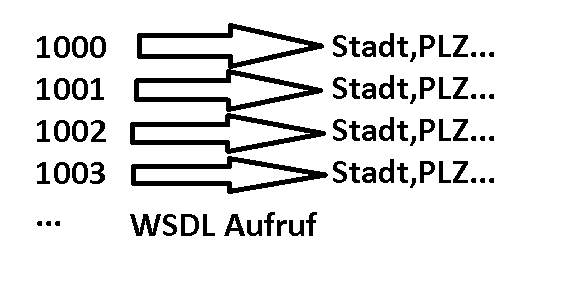
\includegraphics[width=\textheight]{Bilder/presi1.png} 

\end{center}
\end{frame}

\subsection*{Lösungsansatz}

\begin{frame}{Lösungsansatz}
\begin{center}

\begin{itemize}
\item GUI so erstellen, dass zunächst nur Name/Firma angezeigt werden
\item Name/Firma sind bereits nach erstem Webservice Aufruf vorhanden
\item erst nach Klick auf Namen werden Adressdaten via Webservice angefordert
\end{itemize}

\end{center}
\end{frame}

\subsection*{Bild des Lösungsansatzes}

\begin{frame}{Lösungsansatz}
\begin{center}


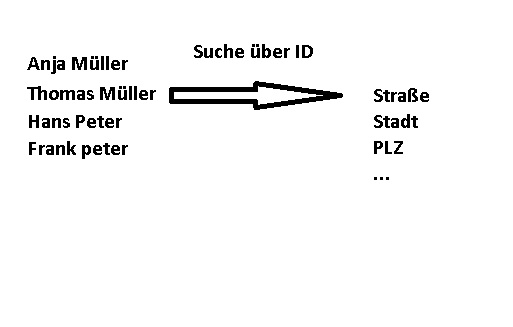
\includegraphics[width=\textheight]{Bilder/presi2.jpg} 

\end{center}
\end{frame}

%%% Google Teil Thorben %%%
\section{Google Connector}
\subsection*{gdata}

\begin{frame}{Die \emph{gdata}-Bibliothek}
 \begin{itemize}
 	\item frei verfügbar (s.\ http://code.google.com/p/gdata-java-client/downloads/list)
 	\item benötigt Account (dli.ides.api@gmail.com)
 	\item kapselt Google-Webservices komplett in \emph{Java}-Klassen
 	\item enthält alle benötigten Klassen und Pakete als JAR-Archive
 \end{itemize}
\end{frame}

\subsection*{Service erstellen}

\begin{frame}[fragile]{Google-Service erstellen (1)}
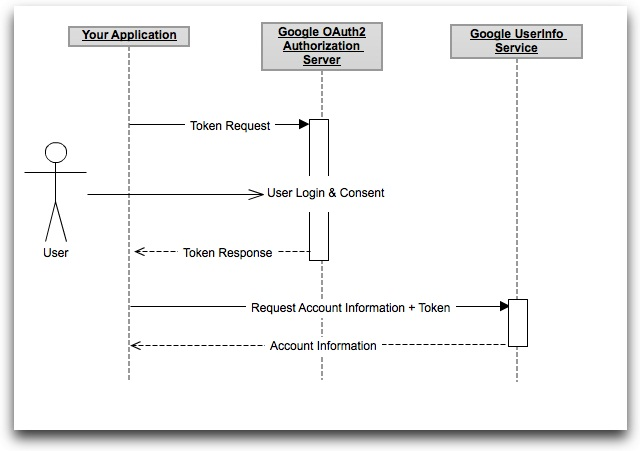
\includegraphics[width=0.9\textwidth]{Bilder/googleOauth.jpg}\\
(Quelle: https://developers.google.com/accounts/docs/OAuth2)
\end{frame}

\begin{frame}[fragile]{Google-Service erstellen (2)}
\begin{block}{Username und Password}
\javalstset
\begin{lstlisting}
ContactsService myService;
myService = new ContactsService(servicename);
try {
	myService.setUserCredentials(username, password);
} catch (AuthenticationException e) {
	e.printStackTrace();
}
\end{lstlisting}
\end{block}
\end{frame}

\subsection*{Create Contact}

\begin{frame}[fragile]{Einen Kontakt erstellen (1)}
\begin{block}{Kontakt-Objekt erstellen}
\javalstset
\begin{lstlisting}
// Create the entry to insert
ContactEntry contact = new ContactEntry();
contact.setTitle(new PlainTextConstruct(contactInfo.getFirstname()
		+ contactInfo.getLastname()));
\end{lstlisting}
\end{block}
\end{frame}

\begin{frame}[fragile]{Einen Kontakt erstellen (2)}
\begin{block}{Namen in ein Kontakt-Objekt einfügen}
\javalstset
\begin{lstlisting}
// Name
Name name = new Name();
name.setFamilyName(new FamilyName(contactInfo.getLastname(), null));
name.setGivenName(new GivenName(contactInfo.getFirstname(), null));
contact.setName(name);
\end{lstlisting}
\end{block}
\end{frame}

\begin{frame}[fragile]{Einen Kontakt erstellen (3)}
\begin{block}{Benutzerdefinierte Einträge zu einem Kontakt-Objekt hinzufügen}
\javalstset
\begin{lstlisting}
// Firma
if (contactInfo.getCompany() != null) {
	ExtendedProperty company = new ExtendedProperty();
	company.setName("Company");
	company.setValue(contactInfo.getCompany());
	contact.addExtendedProperty(company);
}
\end{lstlisting}
\end{block}
\end{frame}

\begin{frame}[fragile]{Einen Kontakt erstellen (4)}
\begin{block}{Das Kontakt-Objekt senden}
\javalstset
\begin{lstlisting}
// Kontakt senden		
URL postUrl = new URL("https://www.google.com/m8/feeds/contacts/
	dli.ides.api@gmail.com/full");
return myService.insert(postUrl, contact);
\end{lstlisting}
\end{block}
\end{frame}

\subsection*{Get Feed}

\begin{frame}[fragile]{Kontakte suchen mit \emph{Queries}}
\begin{block}{Kontakte suchen mit \emph{Queries}}
\javalstset
\begin{lstlisting}
URL feedUrl = new URL("https://www.google.com/m8/feeds/contacts
	/dli.ides.api@gmail.com/full");
Query myQuery = new Query(feedUrl);
ContactFeed resultFeed = null;
// Gruppe
myQuery.setStringCustomParameter("group", "http://www.google.com/m8/feeds/groups
	/dli.ides.api%40gmail.com/base/587c880e884cdacb");
// submit request
resultFeed = myService.query(myQuery, ContactFeed.class);
\end{lstlisting}
\end{block}
\end{frame}

\begin{frame}[fragile]{Kontakte holen}
\begin{block}{Kontakte holen ohne \emph{Queries}}
\javalstset
\begin{lstlisting}
URL feedUrl = new URL("https://www.google.com/m8/feeds/contacts
	/dli.ides.api@gmail.com/full");
resultFeed = myService.getFeed(feedUrl, ContactFeed.class);
\end{lstlisting}
\end{block}
\end{frame}


%%% jABC Teil Dominic %%%
\section{SIB-Programmierung}

\subsection*{}
\begin{frame}{SIB-Programmierung}
	\begin{center}
		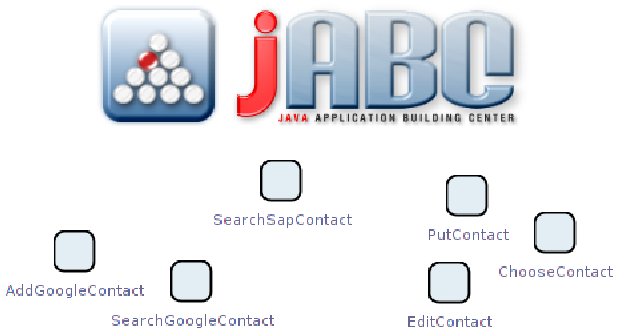
\includegraphics[width=\textheight]{Bilder/titel_sibs.png}
	\end{center}
\end{frame}


\begin{frame}{Vorüberlegungen}
\begin{itemize}[<+->]
	\item \textbf{3 Sorten von SIBs:} Google, SAP, GUI
	\pause
	\item \textbf{Google-SIBs:} Kontakt suchen und hinzufügen
	\item \textbf{SAP-SIB:} Kontakt suchen
	\pause
	\item \textbf{GUI-SIBs:}
		\begin{itemize}[<+->]
			\item Eingabe von Kontakt-Attributen
			\item Auswahl aus einer Liste von Kontakten
		\end{itemize}

\end{itemize}
\end{frame}



\subsection*{SIBs im Detail}
\begin{frame}{Google + SAP: suche Kontakt}
\begin{itemize}[<+->]
	\item \textbf{Input:} eine Instanz der Klasse \texttt{Contact}
		\begin{itemize}[<+->]
			\item dient als Filter für die Suche
		\end{itemize}
	\item \textbf{Output:} Liste von \texttt{Contact}-Objekten

	\item \textbf{Branches:}
		\begin{itemize}[<+->]
			\item \textbf{found:} mehr als 0 Ergebnisse
			\item \textbf{not found:} keine Ergebnisse
			\item \textbf{error:} es wurde eine \textit{Exception} geworfen
		\end{itemize}

\end{itemize}
\end{frame}


\subsection*{SIBs im Detail}
\begin{frame}{Google: Kontakt hinzufügen}
\begin{itemize}[<+->]
	\item \textbf{Input:} eine Instanz der Klasse \texttt{Contact}

	\item \textbf{Output:} keiner

	\item \textbf{Branches:}
		\begin{itemize}[<+->]
			\item \textbf{default:} Kontakt erfolgreich hinzugefügt
			\item \textbf{error:} es wurde eine \textit{Exception} geworfen
		\end{itemize}

\end{itemize}
\end{frame}


\subsection*{SIBs im Detail}
\begin{frame}{GUI: Kontakt-Daten eingeben}
\begin{itemize}[<+->]
	\item \textbf{Input:} eine Instanz der Klasse \texttt{Contact}
		\begin{itemize}[<+->]
			\item Formular wird entsprechend befüllt
			\item zudem Parameter für Fenstertitel und Validierung
		\end{itemize}
	\pause
	\item \textbf{Output:} geänderte(!) Instanz der Klasse \texttt{Contact}
		\begin{itemize}[<+->]
			\item wenn Button "OK" geklickt wurde
		\end{itemize}
	\pause
	\item \textbf{Branches:}
		\begin{itemize}[<+->]
			\item \textbf{ok:} Eingabe bestätigt mit Button "OK"
			\item \textbf{cancel:} Eingabe abgebrochen mit Button "CANCEL"
			\item \textbf{error:} es wurde eine \textit{Exception} geworfen, oder UNKNOWN
		\end{itemize}

\end{itemize}
\end{frame}


\subsection*{SIBs im Detail}
\begin{frame}{GUI: Kontakt-auswählen}
\begin{itemize}[<+->]
	\item \textbf{Input:} Liste von \texttt{Contact}-Objekten
		\begin{itemize}[<+->]
			\item zudem Parameter für Fenstertitel
		\end{itemize}
	\item \textbf{Output:} eine Instanz der Klasse \texttt{Contact}
		\begin{itemize}[<+->]
			\item wenn Button "OK" geklickt wurde
		\end{itemize}

	\item \textbf{Branches:}
		\begin{itemize}[<+->]
			\item \textbf{ok:} Eingabe bestätigt mit Button "OK"
			\item \textbf{cancel:} Eingabe abgebrochen mit Button "CANCEL"
			\item \textbf{error:} es wurde eine \textit{Exception} geworfen, oder UNKNOWN
		\end{itemize}

\end{itemize}
\end{frame}


\subsection*{Probleme im Detail}
\begin{frame}[fragile]{Besonderheit der GUI}
\begin{itemize}[<+->]
	\item \textbf{warten auf Eingabe:} wie \texttt{trace()}-Methode anhalten?
		\begin{itemize}[<+->]
			\item Swing-Frame läuft in einem eigenem Thread!
		\end{itemize}
	\pause
	\item \textbf{Lösung hier:} mittels \texttt{synchronized})-Block in Frame und SIB
\end{itemize}

	\begin{lstlisting}
	public String trace(ExecutionEnvironment env) {

		...
		synchronized (frame) {
			frame.wait();
			...
	\end{lstlisting}

\begin{itemize}[<+->]
	\item \textbf{Vorgehen:}
		\begin{itemize}[<+->]
			\item \texttt{trace()} erstellt den Frame und wartet auf ein \texttt{notify()}
			\item \texttt{notify()} wird vom Action-Listener der Buttons aufgerufen
			\item im Anschluss kann \texttt{trace()} die Eingabe vom Frame erfragen
		\end{itemize}
\end{itemize}
\end{frame}


\subsection*{Probleme im Detail}
\begin{frame}[fragile]{Problem mit jABC}
\begin{itemize}[<+->]
	\item \textbf{eigener Java-Code im jABC:} Unterschiede zum "`normalen"' JRE
	\begin{itemize}[<+->]
			\item Code läuft ausserhalb von jABC...
			\item ABER: Ausführung im Modell wirft Exceptions?
	\end{itemize}
	\pause
	\item \textbf{Lösung hier:} mittels "`bad Practice"'
\end{itemize}
\javalstset
\begin{lstlisting}
...
System.setProperty("javax.xml.parsers.SAXParserFactory", ...);
System.setProperty("javax.xml.parsers.SAXParser", ...);
System.setProperty("oracle.xml.parser.v2.SAXParser", ...);
...
\end{lstlisting}
\begin{itemize}[<+->]
	\item \textbf{Effekt:}
		\begin{itemize}[<+->]
			\item verstellt Optionen der aktiven JVM
			\item auch nach Ausführung des Modells weiterhin wirksam
			\item sollte in realem Szenario vermieden werden
		\end{itemize}
\end{itemize}
\end{frame}


\section{jABC-Modell}

\subsection*{}
\begin{frame}{Modell und Anwendung}
\begin{center}
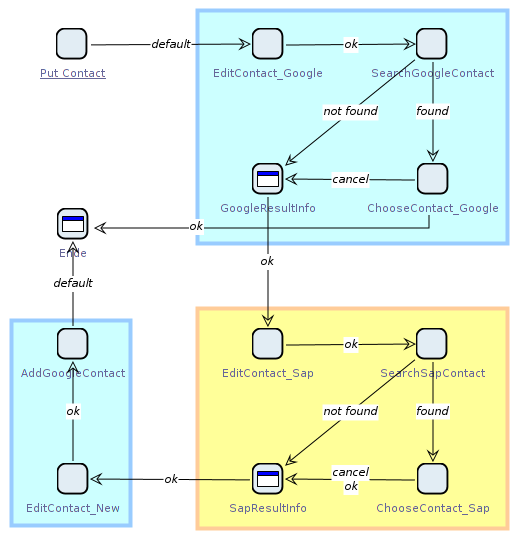
\includegraphics[height=0.8\textheight]{Bilder/jabc_Model.png} 
\end{center}
\end{frame}





\section*{}
\begin{frame}{Vielen Dank f\"ur Ihre Aufmerksamkeit!}
%%%%%%%%%%%%%%	Ende		%%%%%%%%%%%%%%
\tableofcontents
\end{frame}

\end{document}
